\documentclass[10pt,a4paper]{article}
\usepackage[utf8]{inputenc}
\usepackage[italian]{babel}
\usepackage{amsmath}
\usepackage{amsfonts}
\usepackage{amssymb}
\usepackage{graphicx}
\usepackage[left=2cm,right=2cm,top=2cm,bottom=2cm]{geometry}
\newcommand{\rem}[1]{[\emph{#1}]}

\author{Gruppo AC \\ Federico Belliardo, Marco Costa, Lisa Bedini}
\title{Esperienza di Franck-Hertz}
\begin{document}

\maketitle

%Al link http://scipy-cookbook.readthedocs.io/items/SignalSmooth.html è presente una funzione python per eseguire lo smothing i un array 1d di dati, può essere utile per trovare in seguito i massimi locali da associare agli eventi di eccitazione.
%Verificare se sono interspaziati
%Gli elettroni eccitano sempre il primo livello energetico disponibile non arrivano mai ad avere abbastanza energia da eccitare livelli superiori
%Devo guradre i minimi o i massimi?
%Spegare procedura per interpolazione e estrazione di E_A per estrapolazione e calcolo di \lambda
%Acquisizione dati oscilloscopio con il pc

%TODO Ci sono un po' troppe ripetizioni con la scheda dell'esperienza, tutte questi cose preparatorie potrebbero essere saltate e si potrebbe andare direttamente alla descrizione dell'elebaorazione dei dati

\section{Scopo dell'esperienza}
Obiettivo dell'esperienza è dimostrare la struttura discreta dei livelli energetici dell'atomo di neon e di stimarne l'energia di eccitazione mediante lo studio degli effetti dissipativi negli urti anelastici di elettroni su atomi di neon.

\section{Materiale occorrente}
\begin{itemize}
\item Tetrodo a gas neon ELWE U8482230.
\item Sistema di alimentazione e lettura di corrente ELWE.
\item Oscilloscopio.
\end{itemize}

\section{Descrizione esperimento di Franck-Hertz}
L'esperienza prevede lo studio delle collisioni anelastiche elettrone-atomo in un gas di Neon e della relativa fluorescenza indotta dall'eccitazione dei livelli energetici interni. Gli elettroni prodotti per effetto termoionico da un filamento al calor rosso sono accelerati attraverso due griglie di potenziale (tra le quali interagiscono con il neon) e raccolti poi da un anodo dal quale si misura l'intensità di corrente; questo dispositivo è detto tetrodo a gas.
Di seguito è riportato un riassunto della nomenclatura riguardante le tensioni utilizzata nell'esperienza:

\begin{itemize}
%TODO giusto (?)
\item $U_F$: differenza di potenziale applicata al filamento (catodo) rispetto alla terra (?) che ne regola la temperatura, è posta uguale a circa $U_F = 8.0 \,V$ e tenuta costante.
\item $U_G$: differenza di potenziale applicata alla griglia di controllo rispetto al catodo, regola l'estrazione degli elettroni dal metallo per effetto fotoelettrico a freddo (effetto tunnel), questa tensione regola l'emissività del catodo cioè il numero di elettroni emessi per unità di tempo.
\item $U_A$: differenza di potenziale applicata tra il catodo e la griglia anodo al fine di accelerare gli elettroni, nella configurazione a rampa di potenziale questo valore indica il massimo potenziale raggiunto dall'anodo.
\item $U_E$: differenza di potenziale tra la griglia anodo e il collettore applicata al fine di stabilire un campo elettrico frenante per gli elettroni che emergono dall'anodo.
\end{itemize}

Un amplificatore operazionale a transimpedenza fornisce in uscita una tensione proporzionale alla corrente di collettore $I_C$

\begin{figure}[!htb]
  \centering
  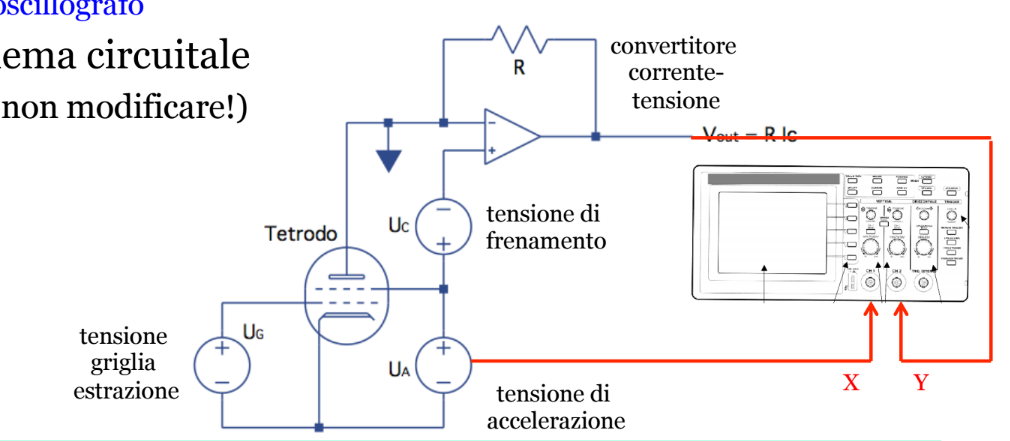
\includegraphics[scale=.5]{circuito.png}
\caption{Schema circuito dell'esperimento e di acquisizione dati.}
\label{circuito}
\end{figure}


\section{Modalità operative}

\section{Osservazioni qualitative}
\begin{itemize}
\item Per un valore fisso di $U_G = \, $ (fisso durante l'esperienza) alla tensione $U_A = \, $ si ottiene la prima luminescenza intono alla griglia anodica. Il parametro $U_G$ regola la sola intensità della luminescenza (a causa del diverso numero di elettroni che fanno urto elastico) ma non influenza il fatto che la luminescenza appaia o meno.
\item Per un valore fisso di $U_A$ (massimo potenziale sull'anodo) il numero minimi e massimi della curva $I_A-U_A$ non cambia ma cambia la sua ampiezza e viene traslata da un valore massimo (corrispondente a $U_E = 0 \, V$) fino a raggiungere lo zero quando vale $U_A = U_E$ cioè ogni elettrone emesso (anche quelli che non hanno interagito con il neon) viene bloccato. In particolare esiste un valore di $U_E$ per cui i minimi della corrente sono a $I_C = 0$ che significa per ogni valore di $U_A$ per cui si ha la creazione di una nuova banda di fluorescenza $U_E$ è sufficiente a bloccare tutti gli elettroni che non hanno interagito o che hanno nuovamente accelerato dopo l'interazione. (cosa succede se aumento  ancora $U_E$ non posso andare sotto 0, probabilmente la curva si rovina).
\item Al diminuire del potenziale $U_E$ è più difficile l'individuazione dei minimi e dei massimi, tuttavia la posizione di questi non varia significativamente al 
variare di $U_E$ 
\end{itemize}
 

\section{Raccolta dati ed elaborazione}

%riporto tabelle grafici e fit, interpolazioni. Fit con parabola intorno ai massimi per trovarli meglio.

Riporto i valori di $U_A$ ai quali si osservano nascere i minimi in modalità manuale

Riporto i grafici di $I_C-U_A$ (massimo numero di oscillazioni) al variare di $U_E$ e relative tabelle che indicano i minimi.

Eseguo un grafico in cui mostro che i minimi e i massimi sono circa costanti al variare di $U_E$

Calcolo il valore medio del minimo al variare di $U_E$ oppure scelgo il valore di $U_E$ per cui le bande di fluorescenza che osservo è visibilmente più nitida (mi sembra un procedimento più sensato.

Calcolo i minimi su ogni grafico eseguendo uno smoothing e prendendo il massimo di un 1D array come mostrato nel link.

Se ho abbastanza punti eseguo fit per calcolare $E_a$ e $\lambda$ e confronto con valore noto, altrimenti concludo dicendo quanto vale l'energia d eccitazione. 

A causa del cammino libero medio $\lambda$ degli elettroni nel gas continuano ad acquisire energia anche quando hanno già raggiunto l'energia di eccitazione. Lo shift di energia rispetto a $E_A$ aumenta all'aumentare del valore di $U_A$ quindi aumenta con il numero del livello che viene eccitato. La differenza tra due massimo consecutivi in funzione del numero quantico principale n è quindi: $E(n) = ( 1 + \frac{\lambda}{L} ( 2 n + 1 ) ) E_A$. 

%Lista script python:
Script che esegue lo smoothing e che calcola minimi e massimi.
Script che plotta i livelli energetici al variare di $U_E$.
Devo prendere manualmente i valori dei massimi e dei minimi e metterli in tre o quattro file differenti.
Script che esegue l'interpolazione lineare.
 

\section{Conclusioni}
%Cerco sul manuale quale è la pressione del neon nell'apparecchio e verico che torna con il libero cammino medio fittato, cerco anche la lunghezza L








\end{document}


